\documentclass[a4paper,11pt,bahasa]{extarticle}
\usepackage[a4paper]{geometry}
\geometry{verbose,tmargin=2cm,bmargin=2cm,lmargin=2cm,rmargin=2cm}

\usepackage{fontspec}
%\defaultfontfeatures{Ligatures=TeX}

%\setmainfont{Linux Libertine O}
%\setmonofont{Fira Mono}
%\setsansfont{Open Sans}

%\setmainfont{Libre Baskerville}
\setmainfont{Georgia}
\setmonofont{Fira Mono}
\setsansfont{Fira Sans}

%\setmainfont{PT Serif}
%\setsansfont{PT Sans}
%\setmonofont{PT Mono}

\setlength{\parindent}{0cm}

\usepackage{amsmath}

\usepackage{setspace}
\onehalfspacing

\usepackage{xcolor}
\usepackage{float}
\usepackage{graphicx}
\usepackage{hyperref}
\usepackage{url}

\usepackage{float}

\usepackage{minted}
%\newminted{verilog}{breaklines}
\newminted{verilog}{breaklines,fontsize=\small}
\newminted{text}{breaklines,fontsize=\small}

\usepackage{babel}

\definecolor{mintedbg}{rgb}{0.95,0.95,0.95}
\usepackage{mdframed}

\BeforeBeginEnvironment{minted}{\begin{mdframed}[backgroundcolor=mintedbg]}
\AfterEndEnvironment{minted}{\end{mdframed}}

\begin{document}

\title{Pengenalan Quartus Prime Lite dan Verilog}
\author{ffr}
\date{}
\maketitle

\tableofcontents

%\section{Mengenai dokumen ini}
%Blah

\section{Pengenalan Quartus Prime}

Quartus Prime merupakan perangkat lunak CAD (computer-assisted design)
yang digunakan untuk desain rangkaian digital. Quartus Prime dikembangkan
oleh Altera. Versi Lite dari Quartus Prime dapat diunduh secara gratis
pada laman Altera\footnote{\url{http://dl.altera.com/?edition=lite}}.
Quartus Prime dapat dijalankan pada
platform Windows dan Linux.
Jendela utama dari Quartus Prime Lite dapat dilihat pada Gambar
\ref{fig:main_window}.

\begin{figure}
\centering
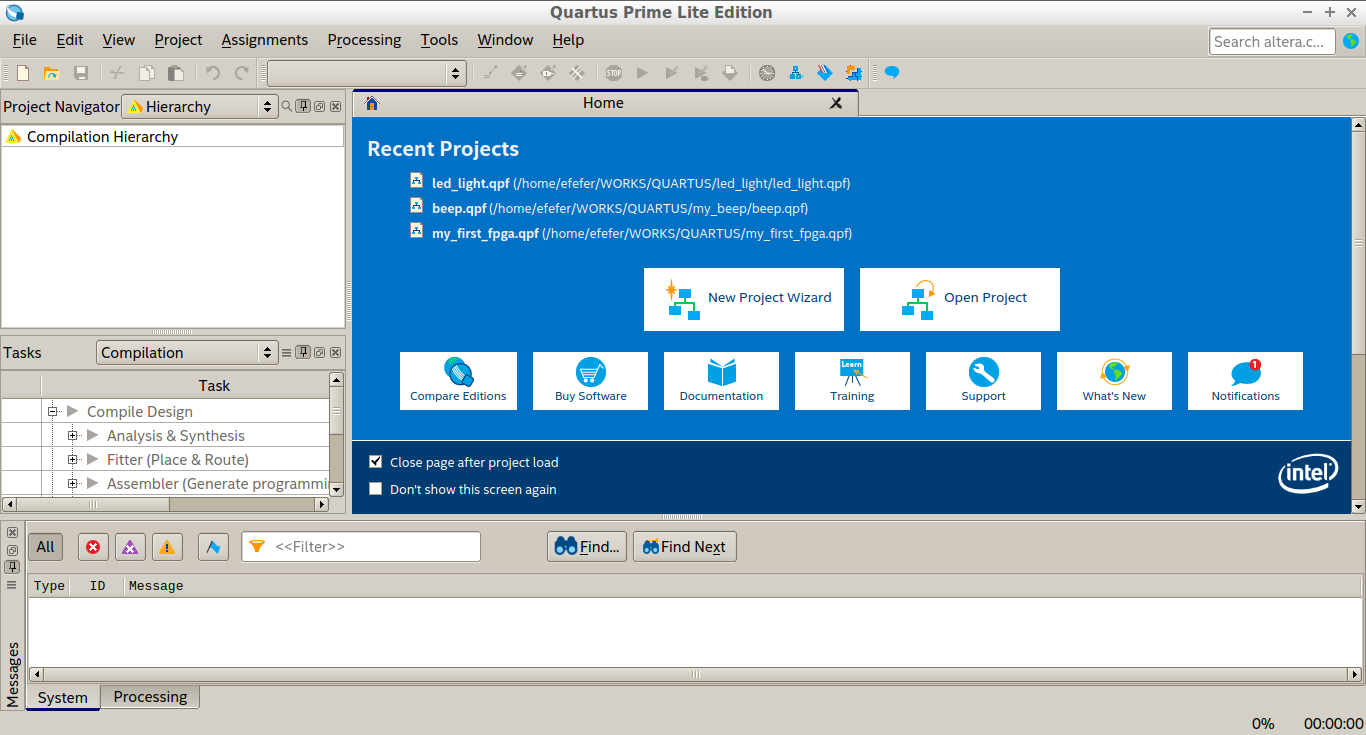
\includegraphics[width=\textwidth]{images/FirstOpen.png}
\par
\caption{Tampilan jendela utama Quartus Prime Lite}\label{fig:main_window}
\end{figure}

Dengan menggunakan CAD, setidaknya ada dua cara untuk
mendesain rangkaian digital:
\begin{itemize}
\item \textit{schematic capture}, dengan membuat skematik dari rangkaian yang
diinginkan.
\item menggunakan Hardware Description Language (HDL).
Dua jenis HDL yang paling populer adalah Verilog dan VHDL.
Kedua bahasa tersebut telah diadopsi sebagai IEEE Standard.
Pada tulisan ini akan digunakan Verilog.
\end{itemize}

\subsection{Membuat project baru}
Berikut ini adalah langkah-langkah yang digunakan untuk membuat New Project
pada Quartus Prime Lite.

\framebox[1.1\width]{\textbf{Langkah 1}}
Pilih menu: \textbf{File $\rightarrow$ New Project Wizard}.
Jendela baru seperti pada gambar berikut akan
muncul.
Centang \textbf{Don't show me this introduction again} jika perlu.
Klik \textbf{Next}.
\begin{figure}[H]
\centering
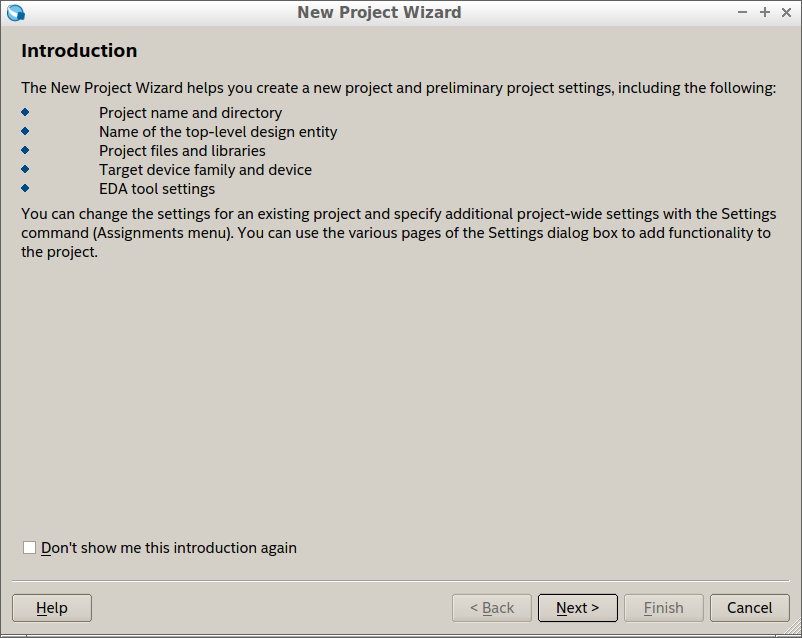
\includegraphics[width=0.5\textwidth]{images/NewProjectWizard_1.png}
\par
\end{figure}


\framebox[1.1\width]{\textbf{Langkah 2}}
Tentukan nama Project yang akan dibuat dan direktori di
mana file-file yang terkait dengan Project ini akan disimpan. Contoh
dapat dilihat pada gambar berikut. Setelah itu, klik \textbf{Next}
setelah semua isian diberikan.

\begin{figure}[H]
\centering
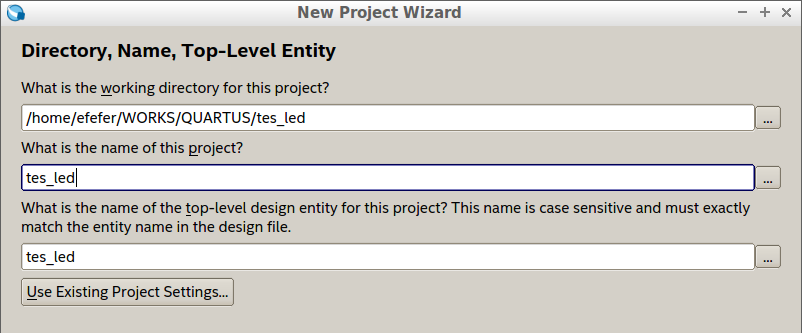
\includegraphics[width=0.5\textwidth]{images/NewProjectWizard_2.png}
\par
\end{figure}


\framebox[1.1\width]{\textbf{Langkah 3}}
Kita diminta untuk memilih jenis Project. Pilih \textbf{Empty Project}.
Setelah itu, klik \textbf{Next}.

\begin{figure}[H]
\centering
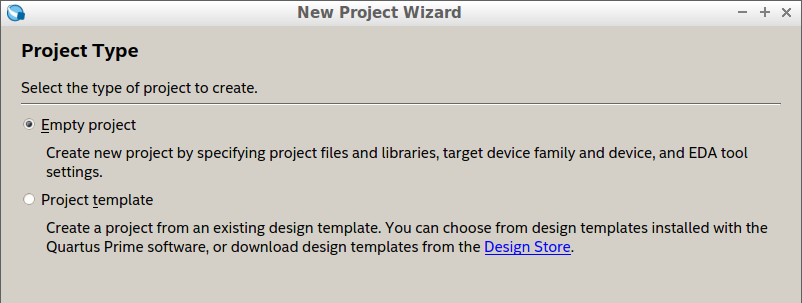
\includegraphics[width=0.5\textwidth]{images/NewProjectWizard_3.png}
\par
\end{figure}


\framebox[1.1\width]{\textbf{Langkah 4}}
Pada langkah ini kita dapat menambahkan file yang sudah ada ke Project
yang akan dibuat. Jika tidak ada langkah ini dapat dilewati.
Klik \textbf{Next}.

\begin{figure}[H]
\centering
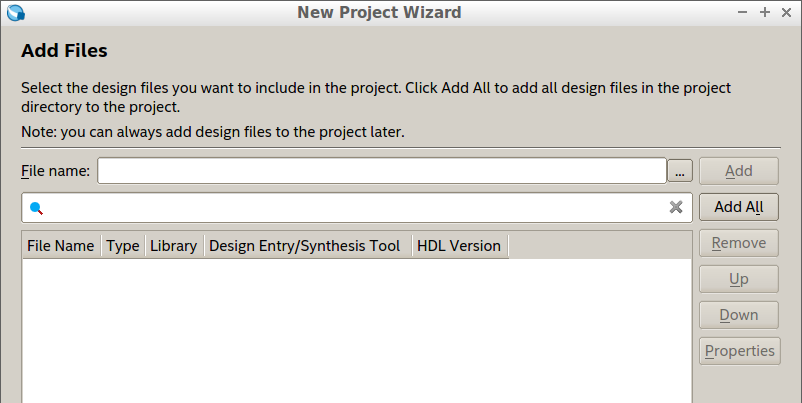
\includegraphics[width=0.5\textwidth]{images/NewProjectWizard_4.png}
\par
\end{figure}

\framebox[1.1\width]{\textbf{Langkah 5}}
Pada langkah ini, kita harus memilih \textbf{Device Family} dan
\textbf{Name}. Untuk \textbf{Device Family} pilih \textbf{Cyclone IV E}.

\begin{figure}[H]
\centering
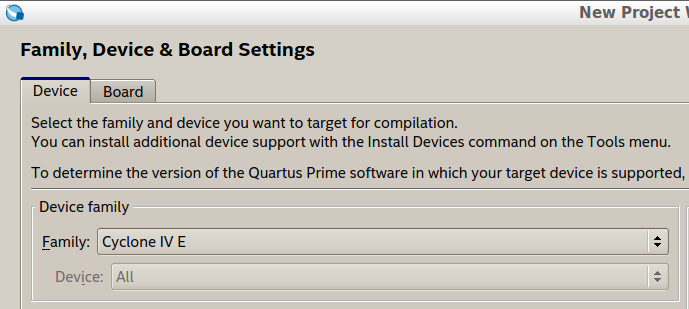
\includegraphics[width=0.5\textwidth]{images/NewProjectWizard_5_device_family.png}
\par
\end{figure}

Pada \textbf{Available Device} pilih \textbf{EP4CE6E22C8}.
Setelah itu, klik \textbf{Next}.

\begin{figure}[H]
\centering
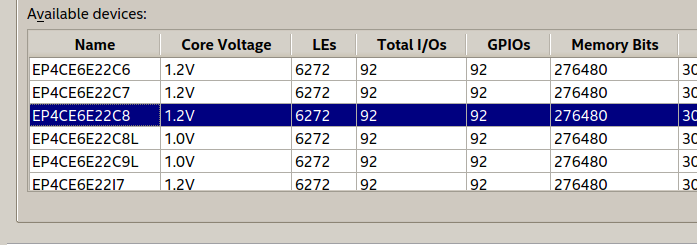
\includegraphics[width=0.5\textwidth]{images/NewProjectWizard_5_device_name.png}
\par
\end{figure}


\framebox[1.1\width]{\textbf{Langkah 6}}
Quartus akan meminta kita untuk memilih setting beberapa tools yang
mungkin digunakan. Untuk sementara pilih \textbf{None} untuk semua tools.
Setelah itu, klik \textbf{Next}.

\begin{figure}[H]
\centering
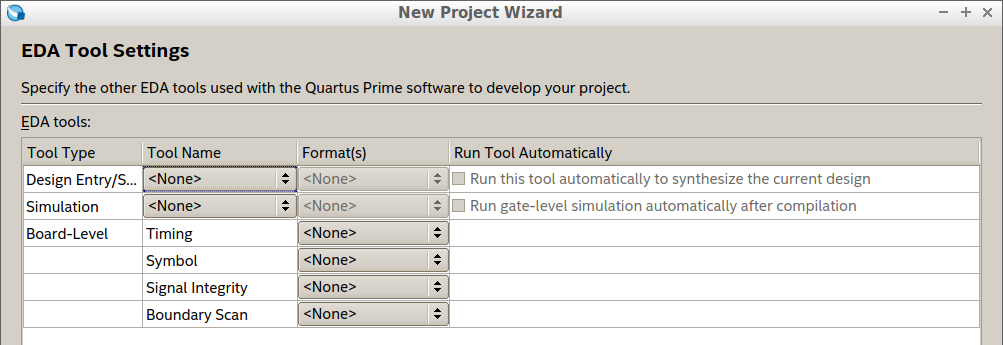
\includegraphics[width=0.5\textwidth]{images/NewProjectWizard_6.png}
\par
\end{figure}

\framebox[1.1\width]{\textbf{Langkah 7}}
Pada bagian akhir, Quartus akan memberikan Summary dari Project yang akan
dibuat. Setelah itu, klik \textbf{Finish}.
\begin{figure}[H]
\centering
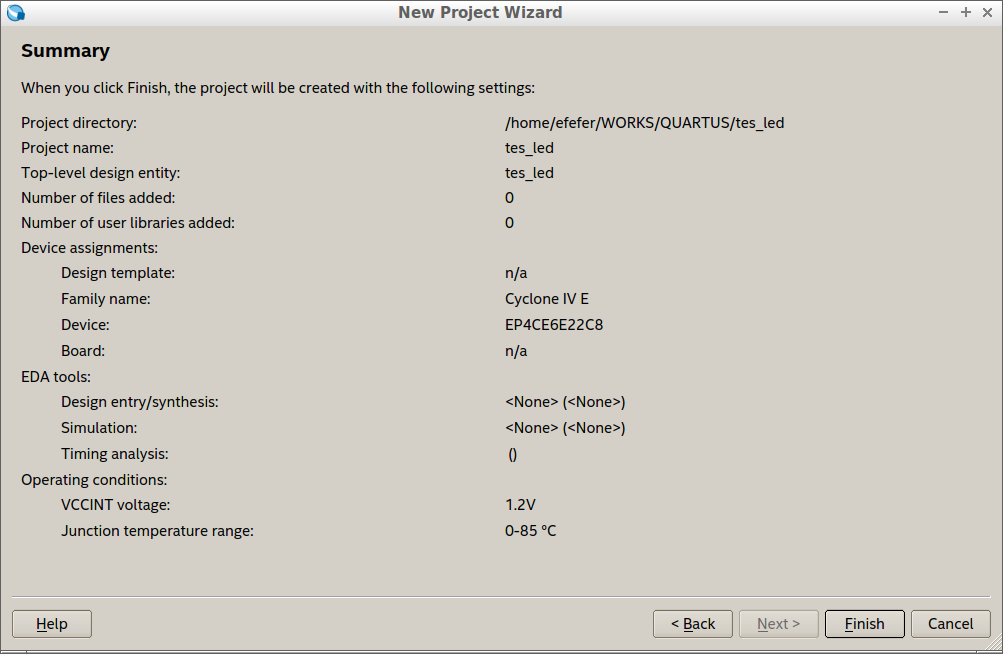
\includegraphics[width=0.5\textwidth]{images/NewProjectWizard_7.png}
\par
\end{figure}



\subsection{Menambahkan skematik baru}

Skematik baru dapat ditambahkan ke dalam project dengan memilih menu
{\sf File $\rightarrow$ New}. Pilih {\sf New Diagram/Schematic File}, kemudian
{\sf OK}.

\begin{figure}[H]
\centering
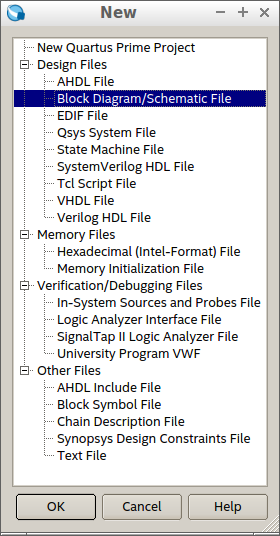
\includegraphics[scale=0.5]{images/NewSchematic.png}
\par
\end{figure}

File skematik kosong akan terbuka pada tab baru dengan nama {\sf Block1.bdf}.
Kita dapat membuat skematik yang kita inginkan pada file ini.

\begin{figure}[H]
\centering
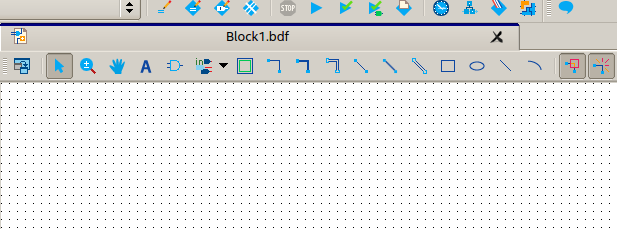
\includegraphics[scale=0.5]{images/EmptySchematic.png}
\par
\end{figure}

Untuk menambahkan komponen, dapat dilakukan dengan cara mengklik toolbar
{\sf Symbol Tool}.

\begin{figure}[H]
\centering
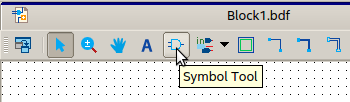
\includegraphics[scale=0.5]{images/SymbolTool.png}
\par
\end{figure}

Komponen yang ingin ditambahkan pada skematik dapat diperoleh dengan
ekspasi node {\sf Libraries}, mencari komponen tersebut, dan memilihnya.
Misalkan kita ingin menambahkan gerbang AND dengan dua input, maka dapat dipilih
pada {\sf primitives $\rightarrow$ logic $\rightarrow$ and2}. Klik
{\sf OK} setelah komponen yang diinginkan telah dipilih.

\begin{figure}[H]
\centering
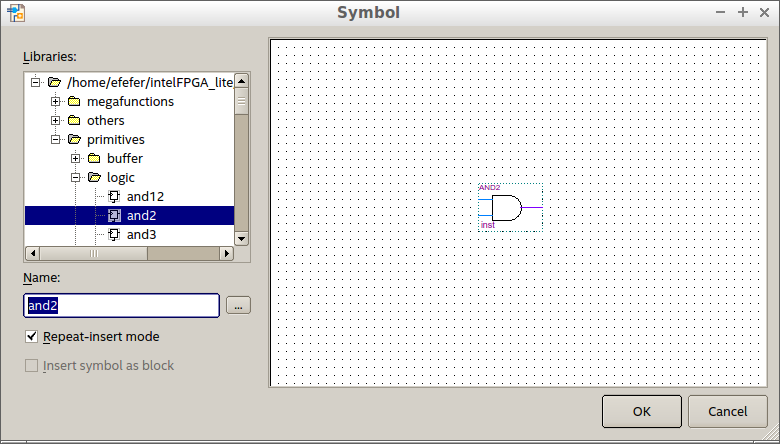
\includegraphics[scale=0.5]{images/BlockAnd.png}
\par
\end{figure}

Pemilihan komponen juga dapat dilakukan dengan mengetikkan nama komponen yang
diinginakan pada isian {\sf Name}, misalnya {\sf jkff} untuk J-K flip-flop.

Khusus untuk menambahkan komponen input dan output, dapat juga digunakan
toolbar {\sf Pin Tool}.
\begin{figure}[H]
\centering
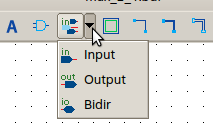
\includegraphics[scale=0.5]{images/PinTool.png}
\par
\end{figure}

Untuk menghubungkan antara satu komponen dengan komponen yang lain, dapat
digunakan {\sf Orthogonal Node Tool}.
\begin{figure}[H]
\centering
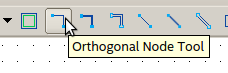
\includegraphics[scale=0.5]{images/OrthogonalNodeTool.png}
\par
\end{figure}

Berikut ini adalah contoh skematik untuk multiplexer 2-to-1:
\begin{figure}[H]
\centering
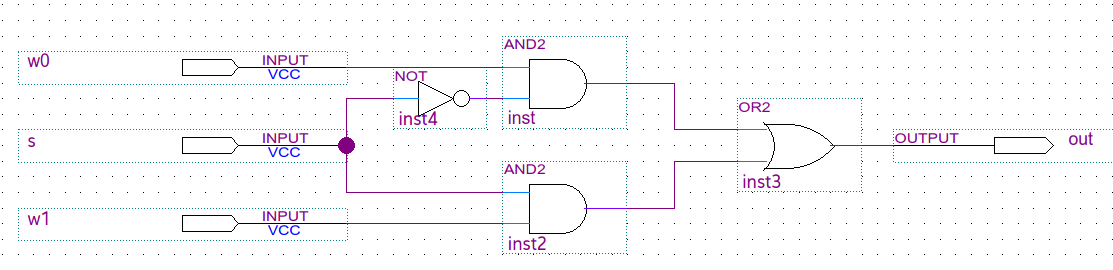
\includegraphics[width=\textwidth]{images/sch_mux_2_1.png}
\par
\end{figure}

Skematik ini kemudian dapat digunakan untuk proses lebih lanjut seperti
simulasi dan download ke hardware FPGA.


\section{Pengenalan Verilog}

\subsection{Sejarah singkat}

Selain menggunakan skematik, desain rangkaian digital juga dapat dilakukan
dengan menggunakan HDL (hardware description language)
seperti Verilog dan VHDL.
Pada kesempatan kali ini kita akan menggunakan Verilog.

Verilog pada awalnya dikembangkan sebagai alat untuk simulasi serta
verifikasi dari rangkaian digital.
Verilog dikembangkan oleh Gateway Design Automation, yang
sekarang menjadi bagian dari Cadence Design Systems.
Pada awal perkembangannya Verilog merupakan bahasa
proprietary, akan tetapi pada
tahun 1990 Verilog dilepaskan ke
domain publik. Sejak saat itu Verilog menjadi salah satu
bahasa yang populer untuk mendeskripsikan rangkaian digital.
Pada tahun 1995 Verilog diadopsi sebagai IEEE Standard, yaitu standard
1364-1995. Pada tahun 2001, versi terbaru dari Verilog yang dikenal dengan
Verilog 2001 diadopsi menjadi IEEE Standard 1364-2001.

\subsection{File Verilog}

Pada Quartus Prime, file Verilog dapat ditambahkan ke Project
dengan memilih menu {\sf File $\rightarrow$ New} dan pilih
{\sf Verilog HDL File}.

\begin{figure}[H]
\centering
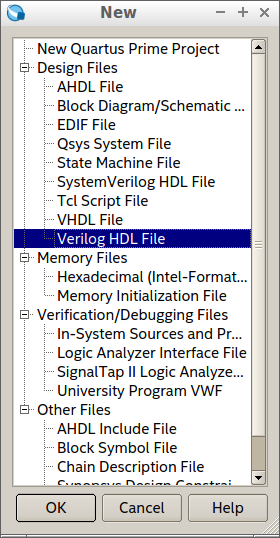
\includegraphics[scale=0.5]{images/new_file_verilog.png}
\par
\caption{New File Verilog HDL}
\end{figure}

File Verilog merupakan file teks sehingga kita dapat menggunakan
teks editor mana saja untuk mengedit file ini.


\subsection{Representasi rangkaian digital dengan Verilog}

Terdapat dua pendekatan untuk mendesain rangkaian digital dengan Verilog:
\begin{itemize}

\item struktural: rangkaian digital dideskripsikan dengan struktur
rangkaian tersebut, membangunnya
dengan elemen-elemen rangkaian seperti gerbang logika, dan mendefisinikan
bagaimana elemen-elemen tersebut saling terhubung satu sama lainnya.

\item perilaku (behavioral): rangkaian digital dideskripsikan dengan
perilaku rangkaian tersebut, bukan dengan struktur rangkaiannya secara
langsung. Pendekatan ini dilakukan dengan menggunakan konstruksi
pemrograman Verilog seperti konstruksi \textbf{if}, \textbf{switch}, dan
\textbf{for} yang juga biasa ditemukan pada bahasa
pemrograman komputer. Kompiler Verilog akan melakukan translasi
dari konstruksi pemrograman tersebut menjadi rangkaian digital yang sesuai.z

\end{itemize}


\subsubsection{Representasi struktural}

Verilog memiliki gerbang logika primitif yang merepresentasikan
gerbang logika yang biasa dipakai pada rangkaian.

Gerbang AND dengan dua input, $x_1$ dan $x_2$,
dan output $y$, misalnya dapat dinyatakan dengan kode Verilog
sebagai berikut.
\begin{verilogcode}
and( y, x1, x2 );
\end{verilogcode}

Gerbang OR dengan 4 input
\begin{verilogcode}
or( y, x1, x2, x3 x4 );
\end{verilogcode}

Inverter $y = \bar{x}$
\begin{verilogcode}
not( y, x );
\end{verilogcode}

Beberapa gerbang primitif pada Verilog dapat diberikan
pada tabel berikut ini.
\begin{table}[h!]
\centering
\begin{tabular}{|ccc|}
\hline
Nama & Deskripsi & Penggunaan \\
\hline\hline
and & $f = (a \cdot b \cdots )$ & \verb|and(f, a, b, ...)| \\
nand & $f = \overline{(a \cdot b \cdots)}$ & \verb|nand(f,a,b,...)| \\
or & $f = (a + b + \cdots)$ & \verb|or(a,b,...)| \\
nor & $f = \overline{(a + b + \cdots)}$ & \verb|nor(a,b,...)| \\
xor & $f = a \oplus b \oplus \cdots $ & \verb|xor(a,b,...)| \\
xnor & $f = a \odot b \odot \cdots $ & \verb|xnor(a,b,...)| \\
not & $f = \bar{a}$ & \verb|not(f,a)| \\
\hline
\end{tabular}
\par
\caption{Beberapa gerbang primitif pada Verilog}
\end{table}

Rangkaian digital yang lebih kompleks
dapat direpresentasikan dengan menggunakan gerbang primitif tersebut.

Dalam tulisan ini, penjelasan mengenai Verilog akan diberikan
melalui contoh.

\begin{figure}[h]
\centering
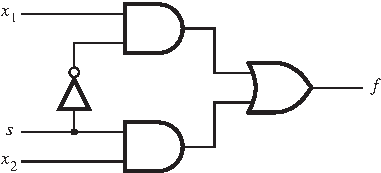
\includegraphics[scale=1.0]{images/fig_2_36.pdf}
\par
\caption{Multiplexer}\label{fig:mux2}
\end{figure}

\framebox[1.1\width]{Contoh 1} Multiplexer pada
Gambar \ref{fig:mux2} dapat dijelaskan dengan kode Verilog berikut.

{\setstretch{1.0}
\begin{verilogcode}
module mux2( x1, x2, s, f );
  input x1, x2, s;
  output f;

  not(k,s);
  and(g,k,x1);
  and(h,s,x2);
  or(f,g,h);
endmodule
\end{verilogcode}
}

Dalam Verilog, rangkaian logika diberikan dalam bentuk modul, didefinisikan
dengan
kata kunci {\tt \textbf{module}}. Suatu modul dapat terdiri dari input dan
output yang disebut sebagai \textit{port}.
Pada contoh di atas, modul dengan nama {\tt \textbf{mux2}} didefinisikan.
Modul {\tt \textbf{mux2}} memiliki 4 port yang bernama {\tt x1}, {\tt x2},
{\tt s}, dan {\tt f}. Pernyataan modul ini diakhiri dengan titik koma.
Pada pernyataan berikutnya, {\tt x1}, {\tt x2} dan {\tt s} dinyatakan
sebagai sinyal input, sedangkan $f$ sebagai sinyal output. Empat baris kode
berikutnya menyatakan struktur dari rangkaian.

Variabel $k$, $g$, dan $h$ tidak dideklarasikan pada kode di atas. Secara default
tipe dari variabel tersebut adalah {\tt wire}.

\framebox[1.1\width]{Contoh 2} Perhatikan rangkaian berikut.

\begin{figure}[H]
\centering
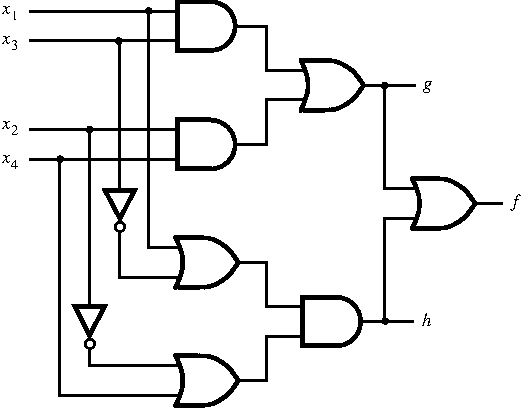
\includegraphics[scale=1.0]{images/fig_2_39.pdf}
\par
\caption{Rangkaian untuk Contoh 2}\label{fig:Contoh2}
\end{figure}

Rangkaian ini memiliki 4 input, yaitu $x_1$, $x_2$, $x_3$, dan
$x_4$, serta 3 output, yaitu $f$, $g$, dan $h$.
Rangkaian ini mengimplementasikan fungsi logika berikut.
\begin{align*}
g & = x_1 x_3 + x_2 x_4 \\
h & = (x_1 + \bar{x_3})(\bar{x_2} + x_4) \\
f & = g + h
\end{align*}

Rangkaian ini dapat diimplementasikan dengan menggunakan kode berikut.
Pada kode ini operator {\tt \textbf{~}} digunakan sebagai pengganti gerbang
NOT.
{\setstretch{1.0}
\begin{verilogcode}
module Contoh2( x1, x2, x3, x4, f, g, h );
  input x1, x2, x3, x4;
  output f, g, h;

  and( z1, x1, x3 );
  and( z2, x2, x4 );
  or( g, z1, z2 );
  or( z3, x1, ~x3 );
  or( z4, ~x2, x4 );
  and( h, z3, z4 );
  or( f, g, h );
endmodule
\end{verilogcode}
}

\subsubsection{Representasi behavioral}

Menggunakan gerbang logika primitif pada Verilog untuk rangkaian yang
kompleks dapat menjadi tugas yang sulit.
Sebagai alternatif, kita dapat menggunakan ekspresi logika dan
level abtraksi yang lebih tinggi
serta kontruksi pemrograman Verilog untuk mendeskripsikan rangkaian
berdasarkan perilaku dari suatu rangkaian.

Sebagai contoh, output dari multiplexer pada Gambar \ref{fig:mux2}
dapat dijelaskan dengan persamaan logika berikut.
\begin{equation*}
f = \bar{s}x_1 + sx_2
\end{equation*}

Dalam Verilog, persamaan ini dapat dinyatakan dengan kode berikut.
{\setstretch{1.0}
\begin{verilogcode}
module mux2_logic_expr( x1, x3, s, f );
  input x1, x2, s;
  output f;

  assign f = ( ~s & x1 ) | ( s & x2 );
endmodule
\end{verilogcode}
}

Pada kode tersebut, operasi AND dan OR dilakukan dengan menggunakan
operator "{\tt\textbf{\&}}" dan "{\tt\textbf{|}}".

Kata kunci {\tt\textbf{assign}} berarti {\it continuous assignment} untuk
sinyal $f$.
Ketika ada sinyal pada ruas kanan yang berubah, maka $f$ akan dievaluasi ulang.
Jika tidak, maka $f$ akan tetap pada nilai sebelumnya.

Dengan menggunakan ekspresi logika, rangkaian pada Gambar \ref{fig:Contoh2}
dapat dituliskan sebagai berikut.
{\setstretch{1.0}
\begin{verilogcode}
module Contoh2_logic_expr( x1, x2, x3, x4, f, g, h );
  input x1, x2, x3, x4;
  output f, g, h;

  assign g = ( x1 &  x3 ) | (  x2 & x4 );
  assign h = ( x1 | ~x3 ) & ( ~x2 & x4 );
  assign f = g | h;
endmodule
\end{verilogcode}
}

Penggunaan ekspresi logika dapat mempermudah penulisan kode Verilog.
Akan tetapi level abstraksi yang lebih tinggi juga dapat digunakan
dengan cara memberikan spesifikasi mengenai perilaku dari rangkaian.
Rangkaian ini juga dapat dideskripsikan dengan menyatakan perilakunya
sebagai berikut.
\begin{itemize}
\item $f = x_1$ jika $s = 0$, dan
\item $f = x_2$ jika $s = 1$
\end{itemize}

Dalam Verilog, perilaku ini dapat dijelaskan dengan menggunakan
pernyataan {\tt \bf if-else} seperti pada kode berikut.
{\setstretch{1.0}
\begin{verilogcode}
module mux2_behavioral( x1, x2, f );
  input x1;
  input x2;
  output f;

  reg f;

  always @(x1 or x2 or s)
    if( s == 0 )
      f = x1;
    else
      f = x2;
endmodule
\end{verilogcode}
}

Beberapa hal yang perlu diperhatikan terkait kode di atas.

\begin{itemize}
\item Pernyataan {\tt\textbf{if-else}} pada Verilog termasuk dalam
\textit{pernyataan prosedural}.
Verilog mengharuskan pernyataan prosedural diletakkan pada blok
{\tt\textbf{always}},
seperti pada kode di atas. Setiap blok {\tt\textbf{always}} dapat terdiri dari satu
pernyataan, seperti pada contoh di atas, atau beberapa pernyataan prosedural.
Suatu modul Verilog dapat memiliki beberapa
blok {\tt\textbf{always}} yang masing-masing blok tersebut menyatakan suatu bagian
dari rangkaian yang sedang dimodelkan.
\item Pernyataan dalam blok {\tt\textbf{always}} akan dievaluasi sesuai dengan urutan yang
diberikan dalam kode. Hal ini kontras dengan pernyataan
\textit{continuous assignment}
yang dievaluasi secara paralel dan tidak bergantung pada urutan yang diberikan
di kode.
\item Pada blok {\tt\textbf{always}}, setelah simbol \textbf{\@},
dalam tanda kurung, disebut
dengan \textit{sensitivity list}. Pernyataan pada blok {\tt\textbf{always}} akan dieksekusi
jika satu atau lebih dari sinyal yang ada pada {\it sensitivity list} berubah.
Hal ini berguna pada waktu simulasi, di mana simulator tidak perlu mengeksekusi
pernyataan setiap waktu.
Untuk keperluan sintesis, \textit{sensitivity list} memberitahu
\textit{compiler} sinyal
apa saja yang secara langsung mempengaruhi keluaran yang diberikan oleh blok
{\tt\textbf{always}}.
\item Jika suatu sinyal diberikan suatu nilai dengan menggunakan pernyataan
prosedural, Verilog mengharuskan sinyal tersebut dideklarasikan sebagai
\textit{variabel}. Hal ini dilakukan dengan cara menggunakan kata kunci
{\tt\textbf{reg}}.
\end{itemize}


\section{Simulasi rangkaian digital dengan Verilog}

Selain menggunakan Quartus Prime, kita juga dapat menggunakan tools lain untuk
mempelajari Verilog. Beberapa tools yang sering digunakan
adalah \textbf{Icarus Verilog} dan \textbf{GTKWave}. Icarus
Verilog adalah compiler Verilog gratis yang dapat digunakan
untuk simulasi rangkaian digital dengan Verilog. Simulasi ini
biasanya menghasilkan output waveform yang dapat divisualisasi dengan
menggunakan GTKWave.

Pada Ubuntu, Icarus Verilog dan GTKWave dapat diinstal dengan menggunakan perintah
\begin{minted}{text}
sudo apt install iverilog gtkwave
\end{minted}
Icarus Verilog dan GTKWave juga dapat digunakan pada sistem operasi Windows.

Kode Verilog yang ditulis untuk simulasi suatu rangkaian digital sering
disebut dengan \textit{textbench}. Modul yang diuji pada simulasi tersebut
disebut sebagai \textit{unit under testing}.

Sebagai contoh pertama, kita akan membuat kode Verilog untuk simulasi
modul {\tt\textbf{mux2}}. Buat file baru dengan nama {\tt test\_mux2.v}
yang isinya sebagai berikut.
\begin{mdframed}[backgroundcolor=mintedbg]
{\setstretch{1.0}
\inputminted[breaklines,fontsize=\small]{verilog}{codes/test_mux2.v}
}\end{mdframed}

Compile file ini dengan Icarus Verilog:
\begin{minted}[fontsize=\small]{text}
iverilog test_mux2.v -o test_mux2
\end{minted}

Perintah ini akan menghasilkan file baru dengan nama {\tt\small test\_mux2}.
File ini merupakan file teks yang dapat dieksekusi dengan perintah {\tt vvp}.
Pada sistem Linux, file ini sudah bersifat \textit{executable} dan dapat dieksekusi
langsung di terminal
\begin{minted}[fontsize=\small]{text}
> ./test_mux2
VCD info: dumpfile test_mux2.vcd opened for output.
  t   i1   i2   s    o
0ns   0    1    1    1
1ns   1    0    1    0
3ns   1    1    1    1
7ns   0    1    0    0
8ns   1    1    0    1
\end{minted}


Berikut ini adalah beberapa penjelasan kode di atas.

\begin{verilogcode}
`timescale 1ns / 1ps
\end{verilogcode}
Baris ini menyatakan bahwa satuan waktu dalam simulasi adalah 1 ns dan
resolusinya adalah 1 ps (0.001 ns).

\begin{verilogcode}
`include "mux2.v"
\end{verilogcode}
Baris ini hanya menyisipkan file {\tt mux2.v} yang berisi definisi dari modul {\tt mux2}.
Baris ini tidak diperlukan apabila \textit{testbench} diberikan pada file yang sama.
Beberapa tools simulasi dapat mencari definisi modul yang diperlukan sehingga
baris ini biasanya juga tidak diperlukan pada kasus tersebut.

\begin{verilogcode}
module test_mux2;
  reg i1, i2, s;
  wire o;
\end{verilogcode}

Baris pertama mendefinisikan suatu modul bernama {\tt\small test\_mux2}. Kode
ini tidak memiliki definisi port karena hanya dimaksudkan sebagai {\it testbench}
untuk modul {\tt\textbf{mux2}}. Pada baris selanjutnya,
tiga sinyal dengan nama {\tt\textbf{i1}}, {\tt\textbf{i2}},
dan {\tt\textbf{s}} dideklarasikan. Tiga sinyal ini nantinya akan menjadi input untuk
modul {\tt\textbf{mux2}}
yang nilainya dapat kita atur nanti.
Sebagai output dari modul {\tt\textbf{mux}}, satu sinyal dengan tipe {\tt\textbf{wire}}
didefinisikan pada baris selanjutnya.

\begin{verilogcode}
  mux2 uut( .x1(i1), .x2(i2), .s(s), .f(o) );
\end{verilogcode}

Pada baris ini, satu \textit{instance} dari modul {\tt\textbf{mux2}} didefinisikan
dengan menggunakan nama $uut$ (\textit{unit under test}).

Kode yang dieksekusi pada awal simulasi diberikan di dalam blok
{\tt\textbf{initial}}.

\begin{verilogcode}
  $dumpfile("test_mux2.vcd");
  $dumpvars(0, test_mux2);
\end{verilogcode}

Dua baris di atas menyatakan bahwa hasil simulasi akan akan ditulis
ke dalam \textit{waveform} yang disimpan pada file {\tt\textbf{test\_mux2.vcd}}.
File ini dapat divisualisasikan dengan menggunakan {\sf GTKWave}.

\begin{verilogcode}
i1 = 1'b0;
i2 = 1'b1;
s  = 1'b1;
\end{verilogcode}

Karena potongan kode di atas diberikan di dalam blok {\tt\textbf{initial}}
maka kode di atas memberikan nilai input {\tt i1}, {\tt i2}, dan {\tt s}
pada saat awal simulasi.

Untuk mengubah nilai dari input pada saat simulasi, dapat digunakan delay
pada blok {\tt\textbf{initial}}, seperti pada baris berikutnya. Delay
dispesifikasikan dengan menggunakan tanda {\tt \#} diikuti dengan lama delay
dalam satuan yang telah dispesifikasikan sebelumnya (ns).

\begin{verilogcode}
#1 i1 = 1'b1; i2 = 1'b0;
#2 i2 = 1'b1;
#4 s  = 1'b0; i1 = 1'b0;
#1 i1 = 1'b1;
#1 $finish;
\end{verilogcode}

Baris terakhir, simulasi akan dihentikan 1ns setelah eksekusi baris sebelumnya.

Kode berikut ini juga berada dalam blok {\tt\textbf{initial}}, akan
tetapi pada blok yang berbeda. Bagian ini
juga dapat diletakkan pada blok {\tt\textbf{initial}}.
Kode ini akan menampilkan hasil simulasi ke terminal.
\begin{verilogcode}
$display("  t   i1   i2   s    o");
$monitor("%1dns   %b    %b    %b    %b", $time, i1, i2, s, o);
\end{verilogcode}

Perintah \verb|$monitor| dan \verb|$display| memiliki kemiripan
dengan \verb|printf| pada bahasa C.

{\color{red} TODO: Contoh simulasi dengan ModelSim}



\section{Eksperimen dengan hardware (FPGA)}

\subsection{Pengenalan IO}

{\color{red} Perlu gambar board FPGA yang akan digunakan}

Beberapa daftar port dari board FPGA yang digunakan:

\begin{table}[H]
\caption{Beberapa port yang digunakan pada board FPGA}\label{tab:pin}
\centering
\begin{tabular}{|c|c|}
\hline 
Clock & PIN\_23\\
\hline 
Reset Push Button & PIN\_25\\
\hline 
Buzzer & PIN\_110 \\
\hline
IR & PIN\_100 \\
\hline 
\multicolumn{2}{|c|}{Push Button}\\
\hline 
key1 & PIN\_88 \\
\hline 
key2 & PIN\_89 \\
\hline 
key3 & PIN\_90 \\
\hline 
key4 & PIN\_91 \\
\hline 
\multicolumn{2}{|c|}{LED} \\
\hline 
LED1 & PIN\_87 \\
\hline 
LED2 & PIN\_86 \\
\hline 
LED3 & PIN\_85 \\
\hline 
LED4 & PIN\_84 \\
\hline 
\end{tabular}
\par
\end{table}



Untuk PIN assignment, buat skematik atau file Verilog terlebih dahulu, kemudian compile.
Buka PIN assignment, set pin yang diperlukan.


\subsubsection{LED}

Assignment nilai boolean ke LED

\subsubsection{Push buttons}

\subsubsection{Seven segments}

\subsubsection{Buzzer}


\subsubsection{Clock}
{\color{red} Berapa frekuensi clock yang digunakan ? 50 MHz ?}

LED blinking (sudah menggunakan counter, implementasinya
mudah pada Verilog)

\subsubsection{IR}
Gunakan kode Verilog yang sudah ada.


\subsection{Rangkaian kombinasional}

XOR

half adder dan full adder

Menyalakan satu atau beberapa LED dengan kombinasi input
4 push button
\begin{itemize}
\item LED1 menyala jika button1 dan button3 ditekan atau button1 dan button 4 ditekan
\item LED2 menyala jika button2 dan button4 ditekan atau button1 ditekan
\end{itemize}





\subsection{Rangkaian sekuensial}

Implementasi D flip-flop

Implementasi J-K flip-flop dan
Toggle operation: buzzer dan LED

register, counter

Kalkulator sederhana, input dari remote IR ?

Rangkaian multiplexing LED

Menampilkan LED perdigit

IR




\appendix

\section{Persiapan USB-Blaster pada Linux}

Diperlukan untuk hardware.

Berikut ini adalah referensi yang dapat digunakan:
{\small
\begin{itemize}
\item \url{https://www.altera.com/support/support-resources/download/drivers/dri-usb_b-lnx.html}
\item \url{http://www.fpga-dev.com/altera-usb-blaster-with-ubuntu/}
\end{itemize}
}

USB Blaster diperlukan untuk mendownload program ke board.

Tidak perlu instalasi driver khusus untuk Linux.

Quartus Prime menggunakan driver \verb|usb_device|
pada Linux untuk mengakses USB-Blaster.

Secara default, yang dapat mengakses USB Blaster adalah root. Agar dapat digunakan
untuk user lain selain root, perlu setting tambahan untuk \verb|udev|.

Hubungkan USB-Blaster ke komputer.

Cek output dari \verb|dmesg| ketika USB-Blaster terhubung ke komputer.
{\small\setstretch{1.0}
\begin{minted}{text}
dmesg | tail
[29293.151196] usb 3-2: new full-speed USB device number 2 using xhci_hcd
[29293.282045] usb 3-2: New USB device found, idVendor=09fb, idProduct=6001
[29293.282056] usb 3-2: New USB device strings: Mfr=1, Product=2, SerialNumber=3
[29293.282061] usb 3-2: Product: USB-Blaster
[29293.282066] usb 3-2: Manufacturer: Altera
[29293.282070] usb 3-2: SerialNumber: 00000000
\end{minted}
}

Cek juga output dari \verb|lsusb|:
{\small\setstretch{1.0}
\begin{minted}{text}
lsusb
Bus 003 Device 002: ID 09fb:6001 Altera Blaster
\end{minted}
}

Berdasarkan output dari \verb|lsusb| diperoleh informasi
sebagai berikut:
{\small\setstretch{1.0}
\begin{minted}{text}
Vendor  ID: 09fb
Product ID: 6001
\end{minted}
}

Buat file baru: {\tt\small /etc/udev/rules.d/51-altera-usb-blaster.rules}
dengan konten sebagai berikut. (perlu akses root)
{\small\setstretch{1.0}
\begin{minted}{text}
SUBSYSTEM=="usb", ATTR{idVendor}=="09fb", ATTR{idProduct}=="6001", MODE="0666"
\end{minted}
}

Kemudian reload {\tt\small udev} (perlu akses root). Lepaskan koneksi USB
Blaster dari komputer sebelum melakukan perintah ini.
{\small
\begin{minted}{text}
udevadm control --reload
\end{minted}
}

Jika tidak ada error, maka seharusnya USB-Blaster dan board yang digunakan sudah
dapat diakses melalui komputer.
Tes apakah sudah dapat FPGA sudah dapat diakses
{\small
\begin{minted}{text}
<quartus_dir>/16.1/quartus/bin/jtagconfig
\end{minted}
}

Sebaiknya langkah berikut ini juga dilakukan agar daemon \verb|jtagd|
dapat mengenali
nama FPGA yang digunakan.
{\small
\begin{minted}{text}
cp <quartus_dir>/16.1/quartus/linux64/pgm_parts.txt /etc/jtagd/jtagd.pgm_parts
\end{minted}
}

Tes apakah FPGA sudah dapat diakses
{\small
\begin{minted}{text}
<quartus_dir>/16.1/quartus/bin/jtagconfig
\end{minted}
}


%{\color{red} XXX: Butuh konfirmasi lebih lanjut mengenai ini}

Perintah {\tt\small jtagconfig} akan secara otomatis menjalankan daemon
{\tt\small jtagd}.
Daemon ini dapat konflik dengan daemon {\tt\small jtagd} yang akan dijalankan
ketika menjalankan Quartus Prime Lite. Untuk amannya, pastikan bahwa
tidak ada daemon {\tt\small jtagd} yang berjalan sebelum menjalankan
Quartus Prime Lite.




\end{document}
